%%%%%%%%%%%%%%%%%%%%%%%%%%%%%%%%%%%%%%%%%%%%%%%%%%%%%%%%%%%%%%%%%%%%%%%%%%%%%%%%
\chapter{Background and Related Work}\label{sec:bg-rw}

\begin{chapterBody}

In this section we summarize the literature concerning educational tooling for
aiding students in code comprehension with a particular regard to expressions.
We also introduce the Expression Tutor platform on top of which all contributions
of this thesis are built upon.

\section{Programming Is Hard}

Learning to program is hard. This has been demonstrated by multiple different
studies such as in \citet{soloway_learning_1986}'s paper about the
``Rainfall problem'' and its follow–up studies
(\citet{mccracken_multi-national_2001, simon_soloways_2013, seppala_we_2015}).
The ``Rainfall problem'', as originally defined~\cite{soloway_learning_1986}, 
consists of
\begin{quote}
Write a program that will read in integers and output their average. Stop
reading when the value 99999 is input.
\end{quote}

It seems a simple and straightforward exercise that students should be expected
to be able to solve after introductory CS courses. The studies highlight how
this is not the case and how these results have been almost constant over the
years. The follow–up studies did not necessarily propose the exact same
exercise as the original Rainfall problem. Sometimes, the exercise was adapted
to better suit the contents that had been covered in the course.
In particular, the study by \citet{mccracken_multi-national_2001}
covers a sample of 216 students from four different universities. 
Instructors participating in the study devised three different simple exercises
revolving around evaluation of arithmetic expressions. Students at the end of
their first year of study, according to instructors, were supposed to be able
to solve these exercise. Students could implement the exercise using the
programming language that they covered during the courses. The solutions were
evaluated using a shared evaluation criteria. The average score was 22.89 out
of 110.

\section{Notional Machines}

In introductory programming CS courses, it is a common practice to make use of
tools such as notional machines to explain concepts to 
students~\cite{donaldson_flexible_2018, aalvik_visast_2019,
fincher_notional_2020}.

A notional machine, according to the definition given by 
\citet{fincher_notional_2020}, is ``a pedagogic device to assist the 
understanding of some aspect of programs or programming''.
One example of a notional machine is the ``Variable as Parking
Space''~\cite{fincher_notional_2020}. This notional machine is aimed at teaching
students the concept of \textit{types} in statically–typed languages.
It represents variables as ``parking spaces'' and their values as ``vehicles''.
Different vehicles are restricted to parking in specific spaces which size
matches. Similarly, different values may only be assigned to variables which
type matches it.
Another notable example of notional machine is the ``Expression as Trees''
(Section~\ref{sec:bg-rw-le-et}). This one helps to reason about expressions,
their composable nature and how they are evaluated.
When dealing with expressions in particular, several tools have been developed
to assist in learning concepts pertaining to them and their 
evaluation~\cite{donaldson_flexible_2018}.
Often these tools involve the use of static analysis to source data that is used
to generate visualizations
(\citet{sirkia_exploring_2014, kumar_effectiveness_2015}).
Another common methodology for working with such visualizations involves the
use of a sequence of sub–languages and build tools around them
(\citet{felleisen_how_2014, henz_stepper_2021}).
These tools usually focus on a singular particular aspect of expressions, such
as operator precedence (\citet{sychev_tool_2022}) and evaluation 
(\citet{clements_modeling_2001}). Sometimes they also employ animations to ease
the understanding of how a program behaves
(\citet{dave_berry_generating_1991}).
Moreover, in the majority of the cases, they all require a certain amount of
``manual work'' to create such activities, limiting the scalability of these
tools.
Because the creation of these exercise is a time–consuming task, and because we
want to create individualized activities for each student, we want to be able
to automate this process.

Studies showcase that, while useful, computer–generated feedback in 
introductory CS courses for students is less impactful than human–supplied
feedback, either from peers or instructors
\cite{leite_effects_2020, pieterse_automated_2013}.
To this end, we will design our the system with the goal to enable instructors
to give better human feedback at scale to students for common misconceptions
and mistakes found during the assessment of the students activities.
At the same time, students immediately receive computer–generated feedback
about the correctness of their submissions.

\section{Expression Trees}\label{sec:bg-rw-le-et}

Expression as Trees is a notional machine that allows to represent and
reason about programming language expressions.
This notional machine showcases the tree structure of expressions, something
that is not always apparent in text–based programming languages.
Expression trees are inspired by compiles Abstract Syntax Trees as used in
compilers. They are the core around which the entire Expression Tutor
platform is built. Expression trees, as seen in
\textbf{Figure~\ref{fig:bg-etree}}, represent different values and
operators of expressions in nodes that are connected together by edges.
Nodes may also be annotated with a type and an evaluated value.

\begin{figure}[ht]
\centering
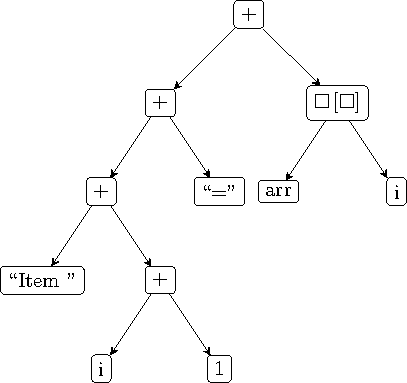
\includegraphics[height=.3\textwidth]{res/2/expression_tree_generic.pdf}
\caption{Expression tree visualization of the Java expression\\
\lstinline[language=Java]{"Item " + (i + 1) + "=" + arr[i]}}
\label{fig:bg-etree}
\end{figure}

\section{Expression Tutor}

Expression Tutor is an educational platform, primarily accessible through its
website~\cite{matthias_hauswirth_expression_2023} that helps learning the
concept of expressions in programming languages by providing worked examples,
documentation and activities built around the Expression as Trees notional
machine.

\textbf{Figure~\ref{fig:bg-et-analyzer}} showcases how Expression Tutor can
analyze Java source code and display the Expression trees for each expression
that was found. \textbf{Figure~\ref{fig:bg-et-we}} displays one of the worked
examples available on the website that explains Church booleans in the untyped
lambda calculus language (as defined in Section~5.2 of the book Types and 
Programming Languages~\cite{pierce_types_2002}) using expression trees.

\begin{figure}[ht]
\centering
\includegraphics[width=0.5\textwidth]{res/2/expression_tree.png}
\caption{Expression tree diagram visualization of the Java expression
\hfill\break
\lstinline[language=Java]{"Item " + (i + 1) + "=" + arr[i]}}
\label{fig:bg-etd}
\end{figure}

\begin{figure}[ht]
    \centering
    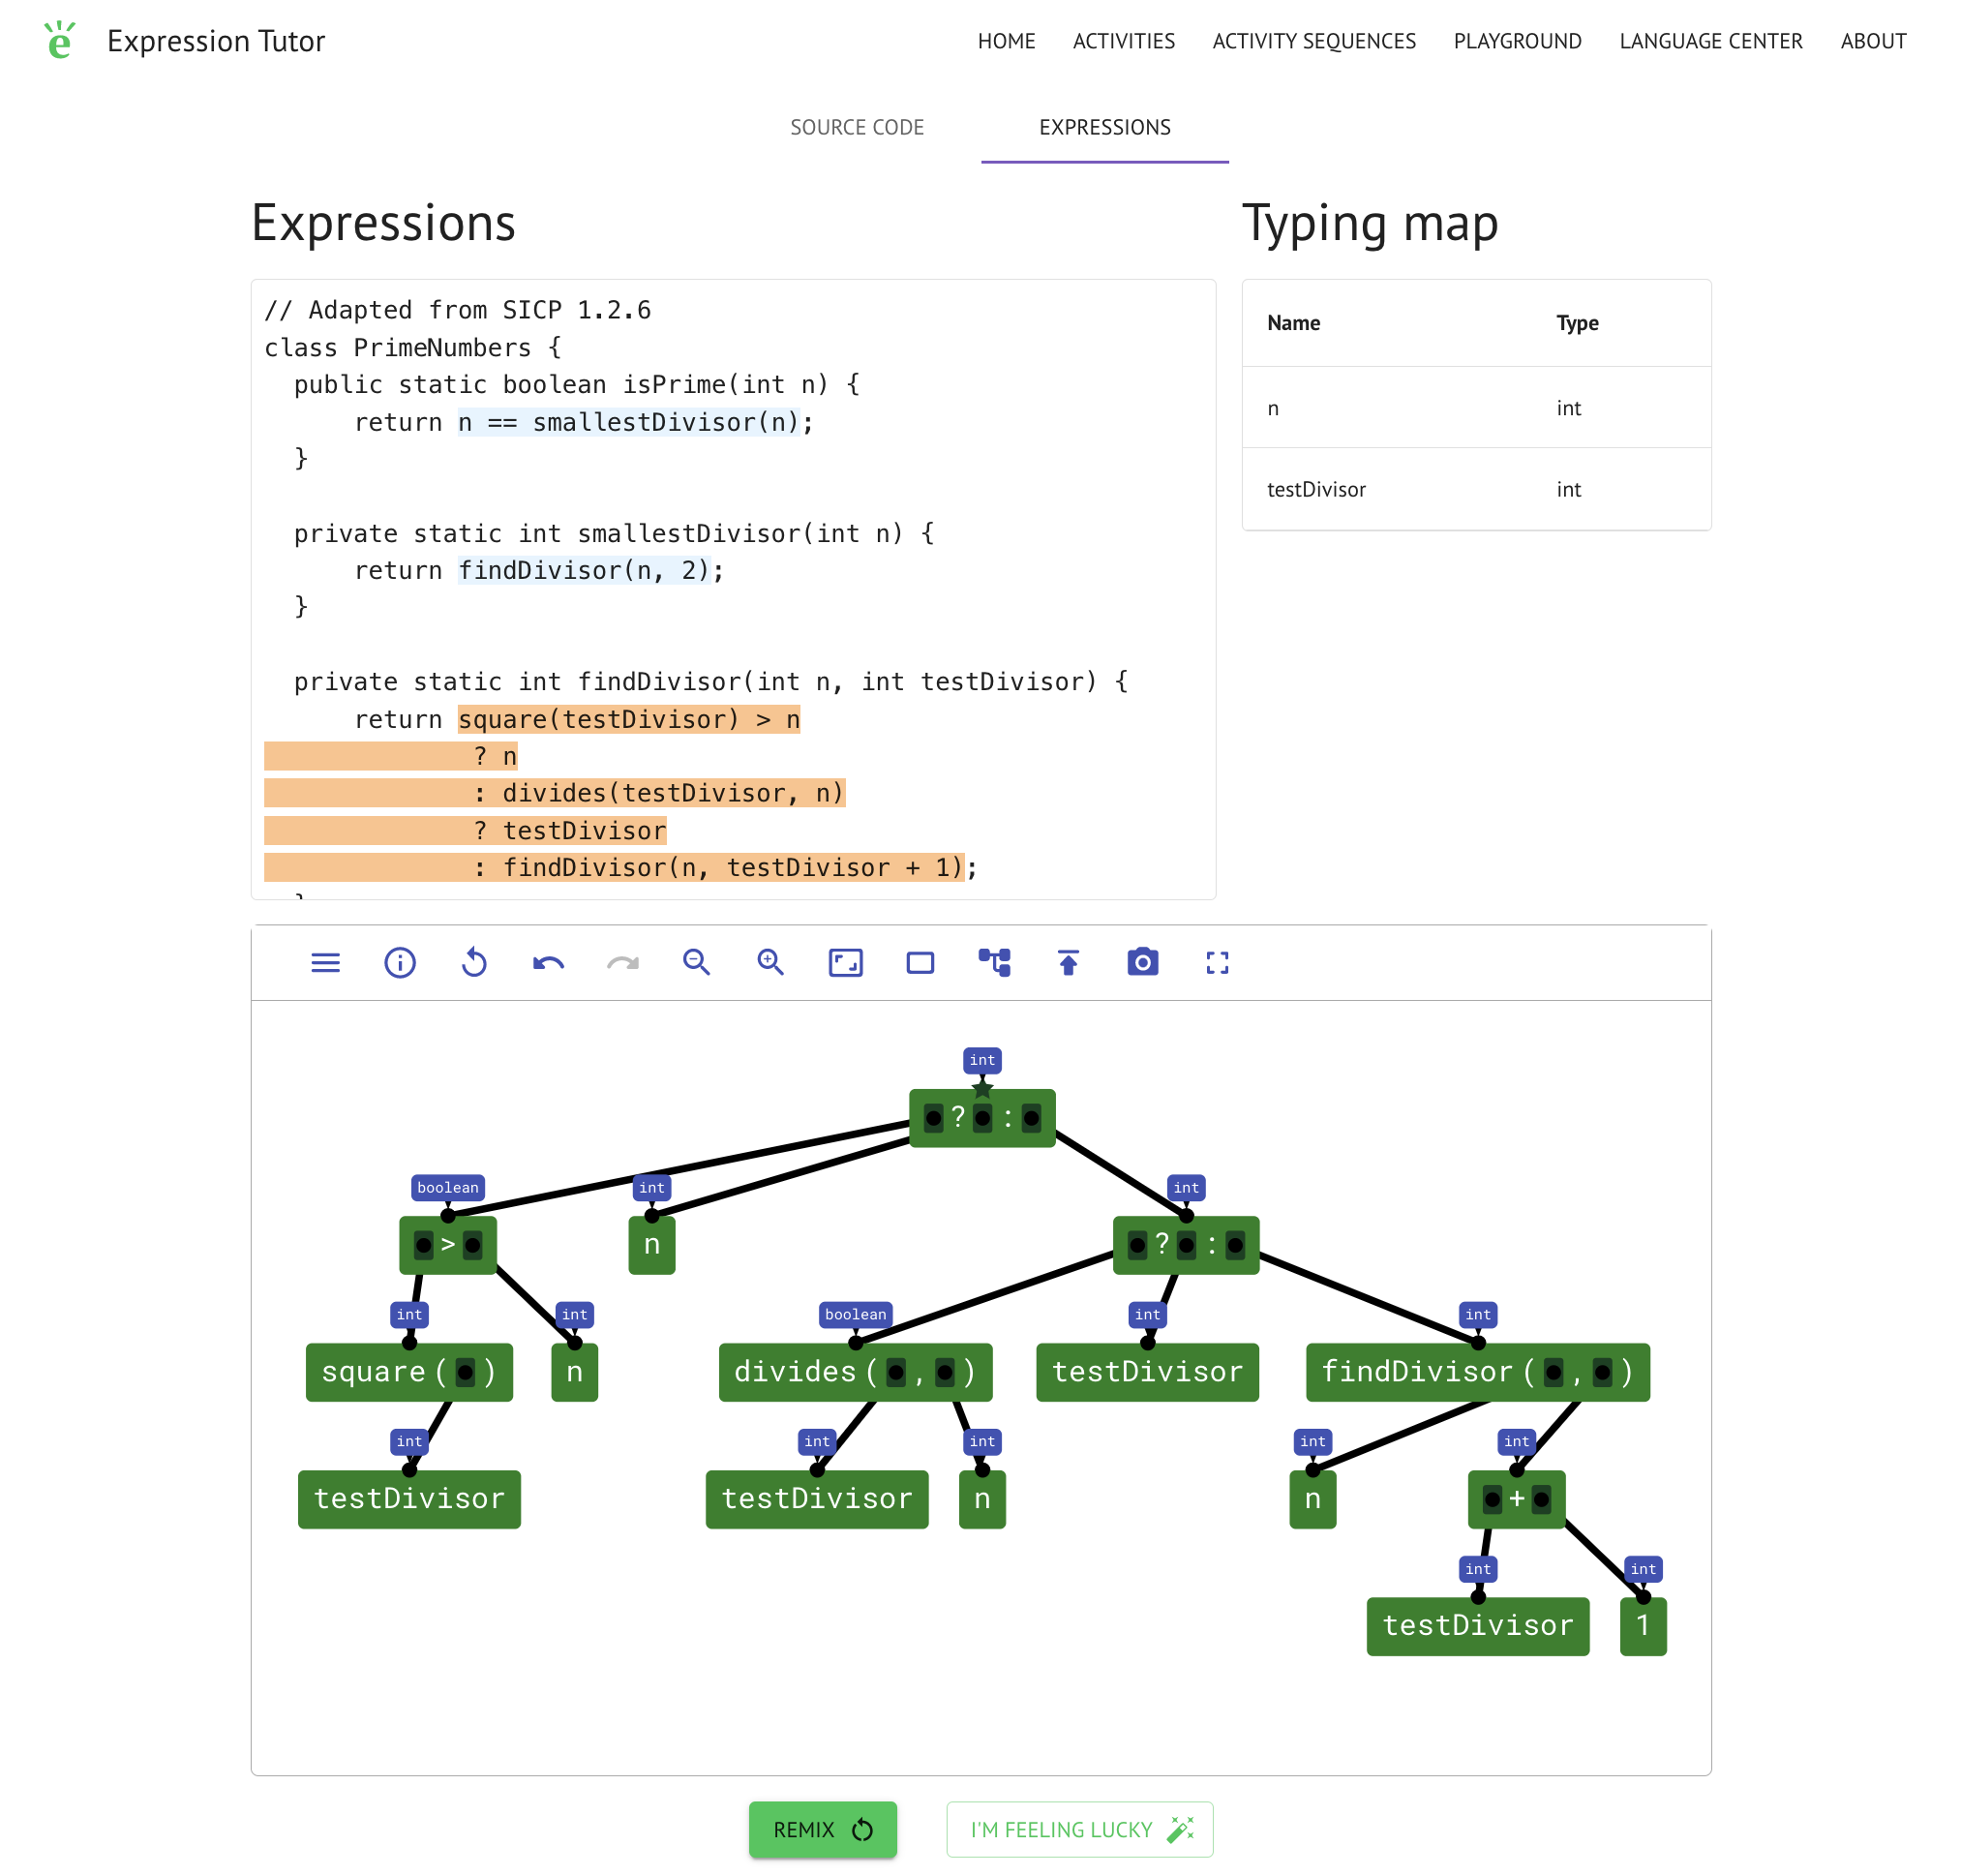
\includegraphics[width=0.8\textwidth]{res/2/et_analyzer.png}
    \caption{The expression analyzer can generate expression trees for each
expression found in the Java file.}
    \label{fig:bg-et-analyzer}
\end{figure}

\begin{figure}[ht]
    \centering
    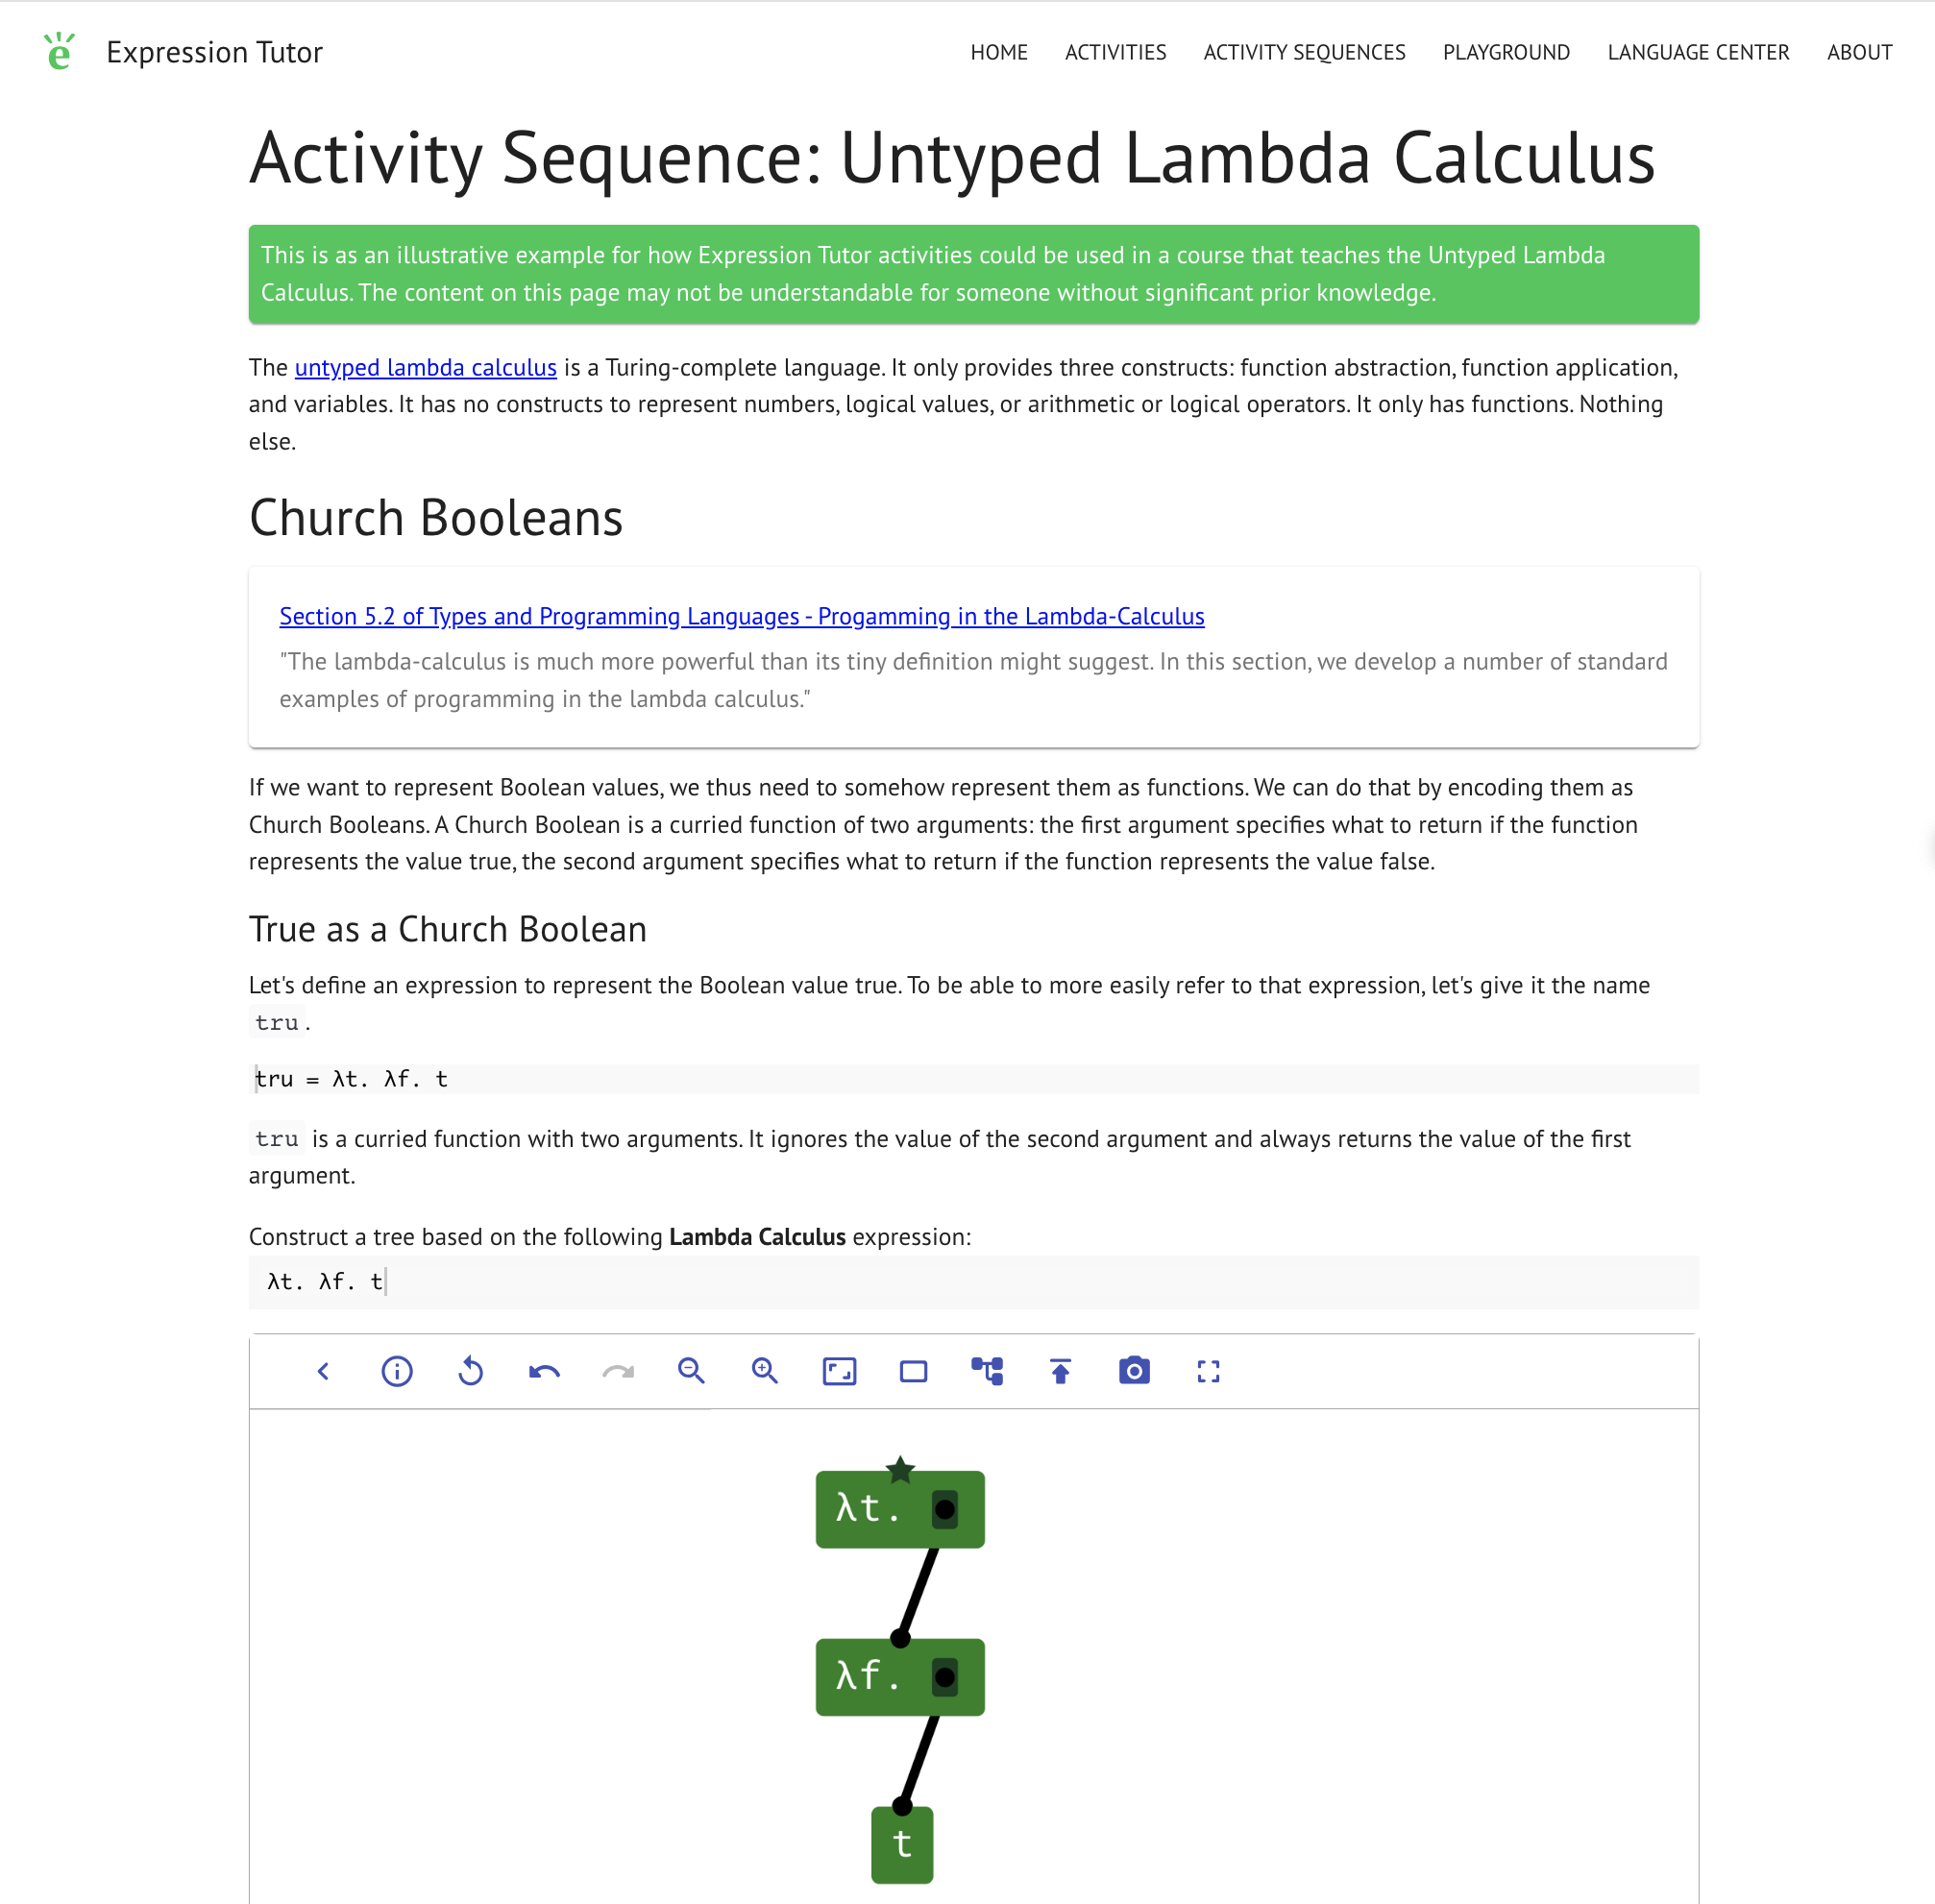
\includegraphics[width=0.8\textwidth]{res/2/et_worked_example.png}
    \caption{Worked example that explains Church booleans using the
Expressions as Trees notional machine.}
    \label{fig:bg-et-we}
\end{figure}

\subsection{Expression Tree Diagram}\label{sec:bg-et-etd}

Starting from the representation of the notional machine, we adopt a data
structure that allows to encode the expression trees as they would have been
written on a medium such as paper or whiteboard.
While a correct solution in this notional machine should always be a tree, the
data structure needs to be a graph. By allowing cycles and
more free connections between nodes, it becomes possible to represent
a variety of students' mistakes. With a tree–like data structure, it would have
been impossible to capture Expression \textit{Trees} that contain cycles or
edges with shared endpoints. These mistakes have been observed and catalogued
by~\citet{chiodiniCuratedInventoryProgramming2021} while grading expression
trees drawn by students on paper.
\textbf{Figure~\ref{fig:bg-et-etd-incorrect}} depicts some of the situations
that would be impossible to represent with a well–formed tree data structure.
We call this data structure ``expression tree diagram''
(\textbf{Figure~\ref{fig:bg-etd}}).

\begin{figure}[ht]
    \centering
    \begin{subfigure}[b]{0.3\textwidth}
        \centering
        \includegraphics[height=3em]{res/2/etd_loop.png}
        \caption{Cycle.}
    \end{subfigure}
    \begin{subfigure}[b]{0.3\textwidth}
        \centering
        \includegraphics[height=3em]{res/2/etd_unplugged_hole.png}
        \caption{Empty hole.}
    \end{subfigure}
    \begin{subfigure}[b]{0.3\textwidth}
    \centering
        \includegraphics[height=6em]{res/2/etd_shared_plug.png}
        \caption{Multiple children in hole.}
    \end{subfigure}
    \caption{Well–formedness mistakes.}
    \label{fig:bg-et-etd-incorrect}
\end{figure}

The expression tree diagram data structure is the language–agnostic 
representation of expression trees used across the Expression Tutor platform.
expression tree diagrams are not tied to any particular programming language,
as long as there exists some partial mapping from the programming language 
source code to an expression tree diagram.

The edges connect a ``node plug'' to a \textit{hole} within another node. This
representation differs from the conventional way of connecting tree nodes by
drawing edges between them because it provides information about the position 
of the connected component with regards to the other textual components of a
node. It is necessary to correctly showcase the composable nature of
expressions.

\subsubsection*{Implementation}

A diagram (composed of \texttt{Edge}s and \texttt{Node}s) represents
expression trees. 

\texttt{Nodes} are made of the following:

\begin{itemize}
    \item \texttt{nodePlug}: a plug used to connect the node to a plug in
another Node through an Edge. Usually graphically represented at the top of
the Node.
    \item \texttt{contents}: the contents of the Node. An ordered sequence of
\texttt{NodeContentElem}s (node content elements).
    \item \texttt{type}: an optional label that represents the type of the
sub–expression represented by the Node.
    \item \texttt{value}: an optional label that represent the value of the
sub–expression represented by the Node.
\end{itemize}

A \texttt{NodeContentElem} is one of:

\begin{itemize}
    \item \texttt{Hole}: allows to connect this Node to another one
(\textit{parent} expression to the sub–expression) through an Edge.
A Hole contains a Plug, just like the one found in the \texttt{nodePlug}.
    \item \texttt{NameDef}: is the abbreviation of ``name definition'', a
terminology commonly used by compilers at ``name analysis'' stage.
    \item \texttt{NameUse}: is the abbreviation of ``name usage'', a
terminology commonly used by compilers at ``name analysis'' stage.
    \item \texttt{Other}: represent textual content. Includes tokens
that are not a name, such as literals, keywords and special tokens. 
\end{itemize}

A \texttt{Plug} is a pair of integers. The first integer is an
identifier for the node the plug belongs to and it is guaranteed to
be unique within the current expression tree diagram. The second
integer is used to distinguish the Plug among all plugs of the Node.
The node top plug is usually the one which has the second value equal to 0.

An \texttt{Edge} is simply defined as a pair of \texttt{Plugs}.

\textbf{Figure~\ref{fig:bg-etd-node}} illustrates the various components
of a node of an Expression Tree Diagram, while
\textbf{Figure~\ref{fig:uml-etd}} shows the UML diagram for the
\texttt{ExprTreeDiagram} data structure.

\begin{figure}[ht]
    \centering
    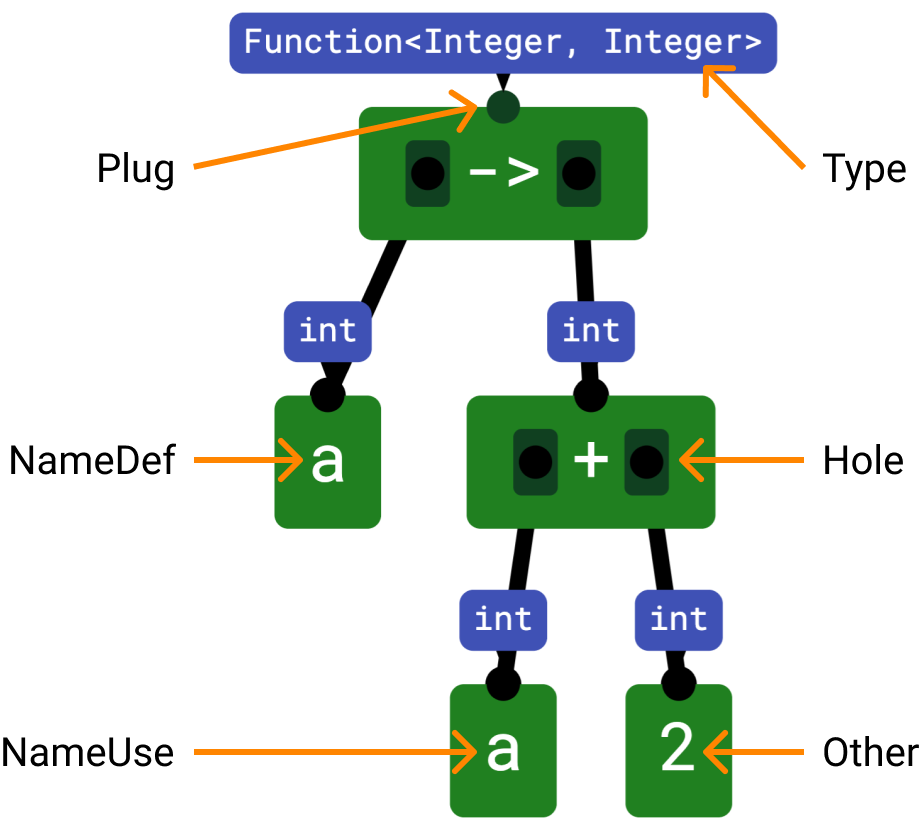
\includegraphics[width=0.5\textwidth]{res/2/etd_contents.png}
    \caption{The various contents of a node for the expression tree diagram of
the Java expression \lstinline[language=Java]{a -> a + 2}.}
    \label{fig:bg-etd-node}
\end{figure}

\begin{figure}[ht]
\centering
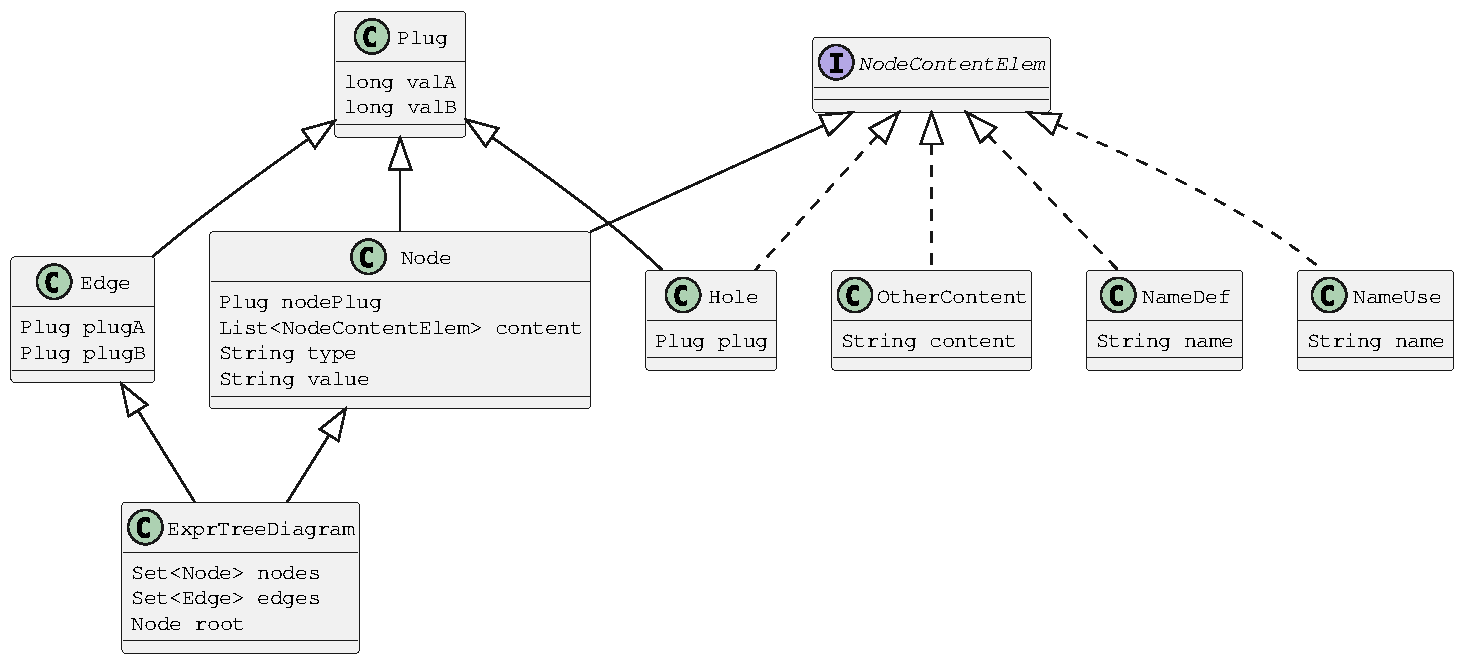
\includegraphics[width=0.8\textwidth]{res/2/etd_uml.pdf}
\caption{UML diagram of the expression tree diagram data structure.}
\label{fig:uml-etd}
\end{figure}

\subsection{Expression Tutor Activities}

Expression Tutor supports various activities that can be performed on
the Expression Tutor website.
Students are provided a code snippet for an expression and are tasked to
draw the corresponding expression tree. This exercise works towards the 
following learning goals:

\begin{enumerate}
    \item Given an expression, decompose it into sub–expressions.
    \item Given an expression, determine its type and explain possible
type errors.
\end{enumerate}

Similarly to Parson problems~\cite{parsons_parsons_2006}, students are
not required to create everything from scratch. Rather, they are provided
the basic \textit{building blocks} (in this case a number of nodes) to be
used to compose the expression tree.
The instructor usually prepares such activities manually, creating all the
required nodes alongside with \textit{distractors}. These are vital to
assess the achievement of the learning goals, because having extra wrong
choices opens up more opportunities for mistakes and for students to express
their misconceptions.
These activities are then saved on the platform and submitted to the instructor,
who has to manually check and grade them.

\begin{figure}[ht]
    \centering
    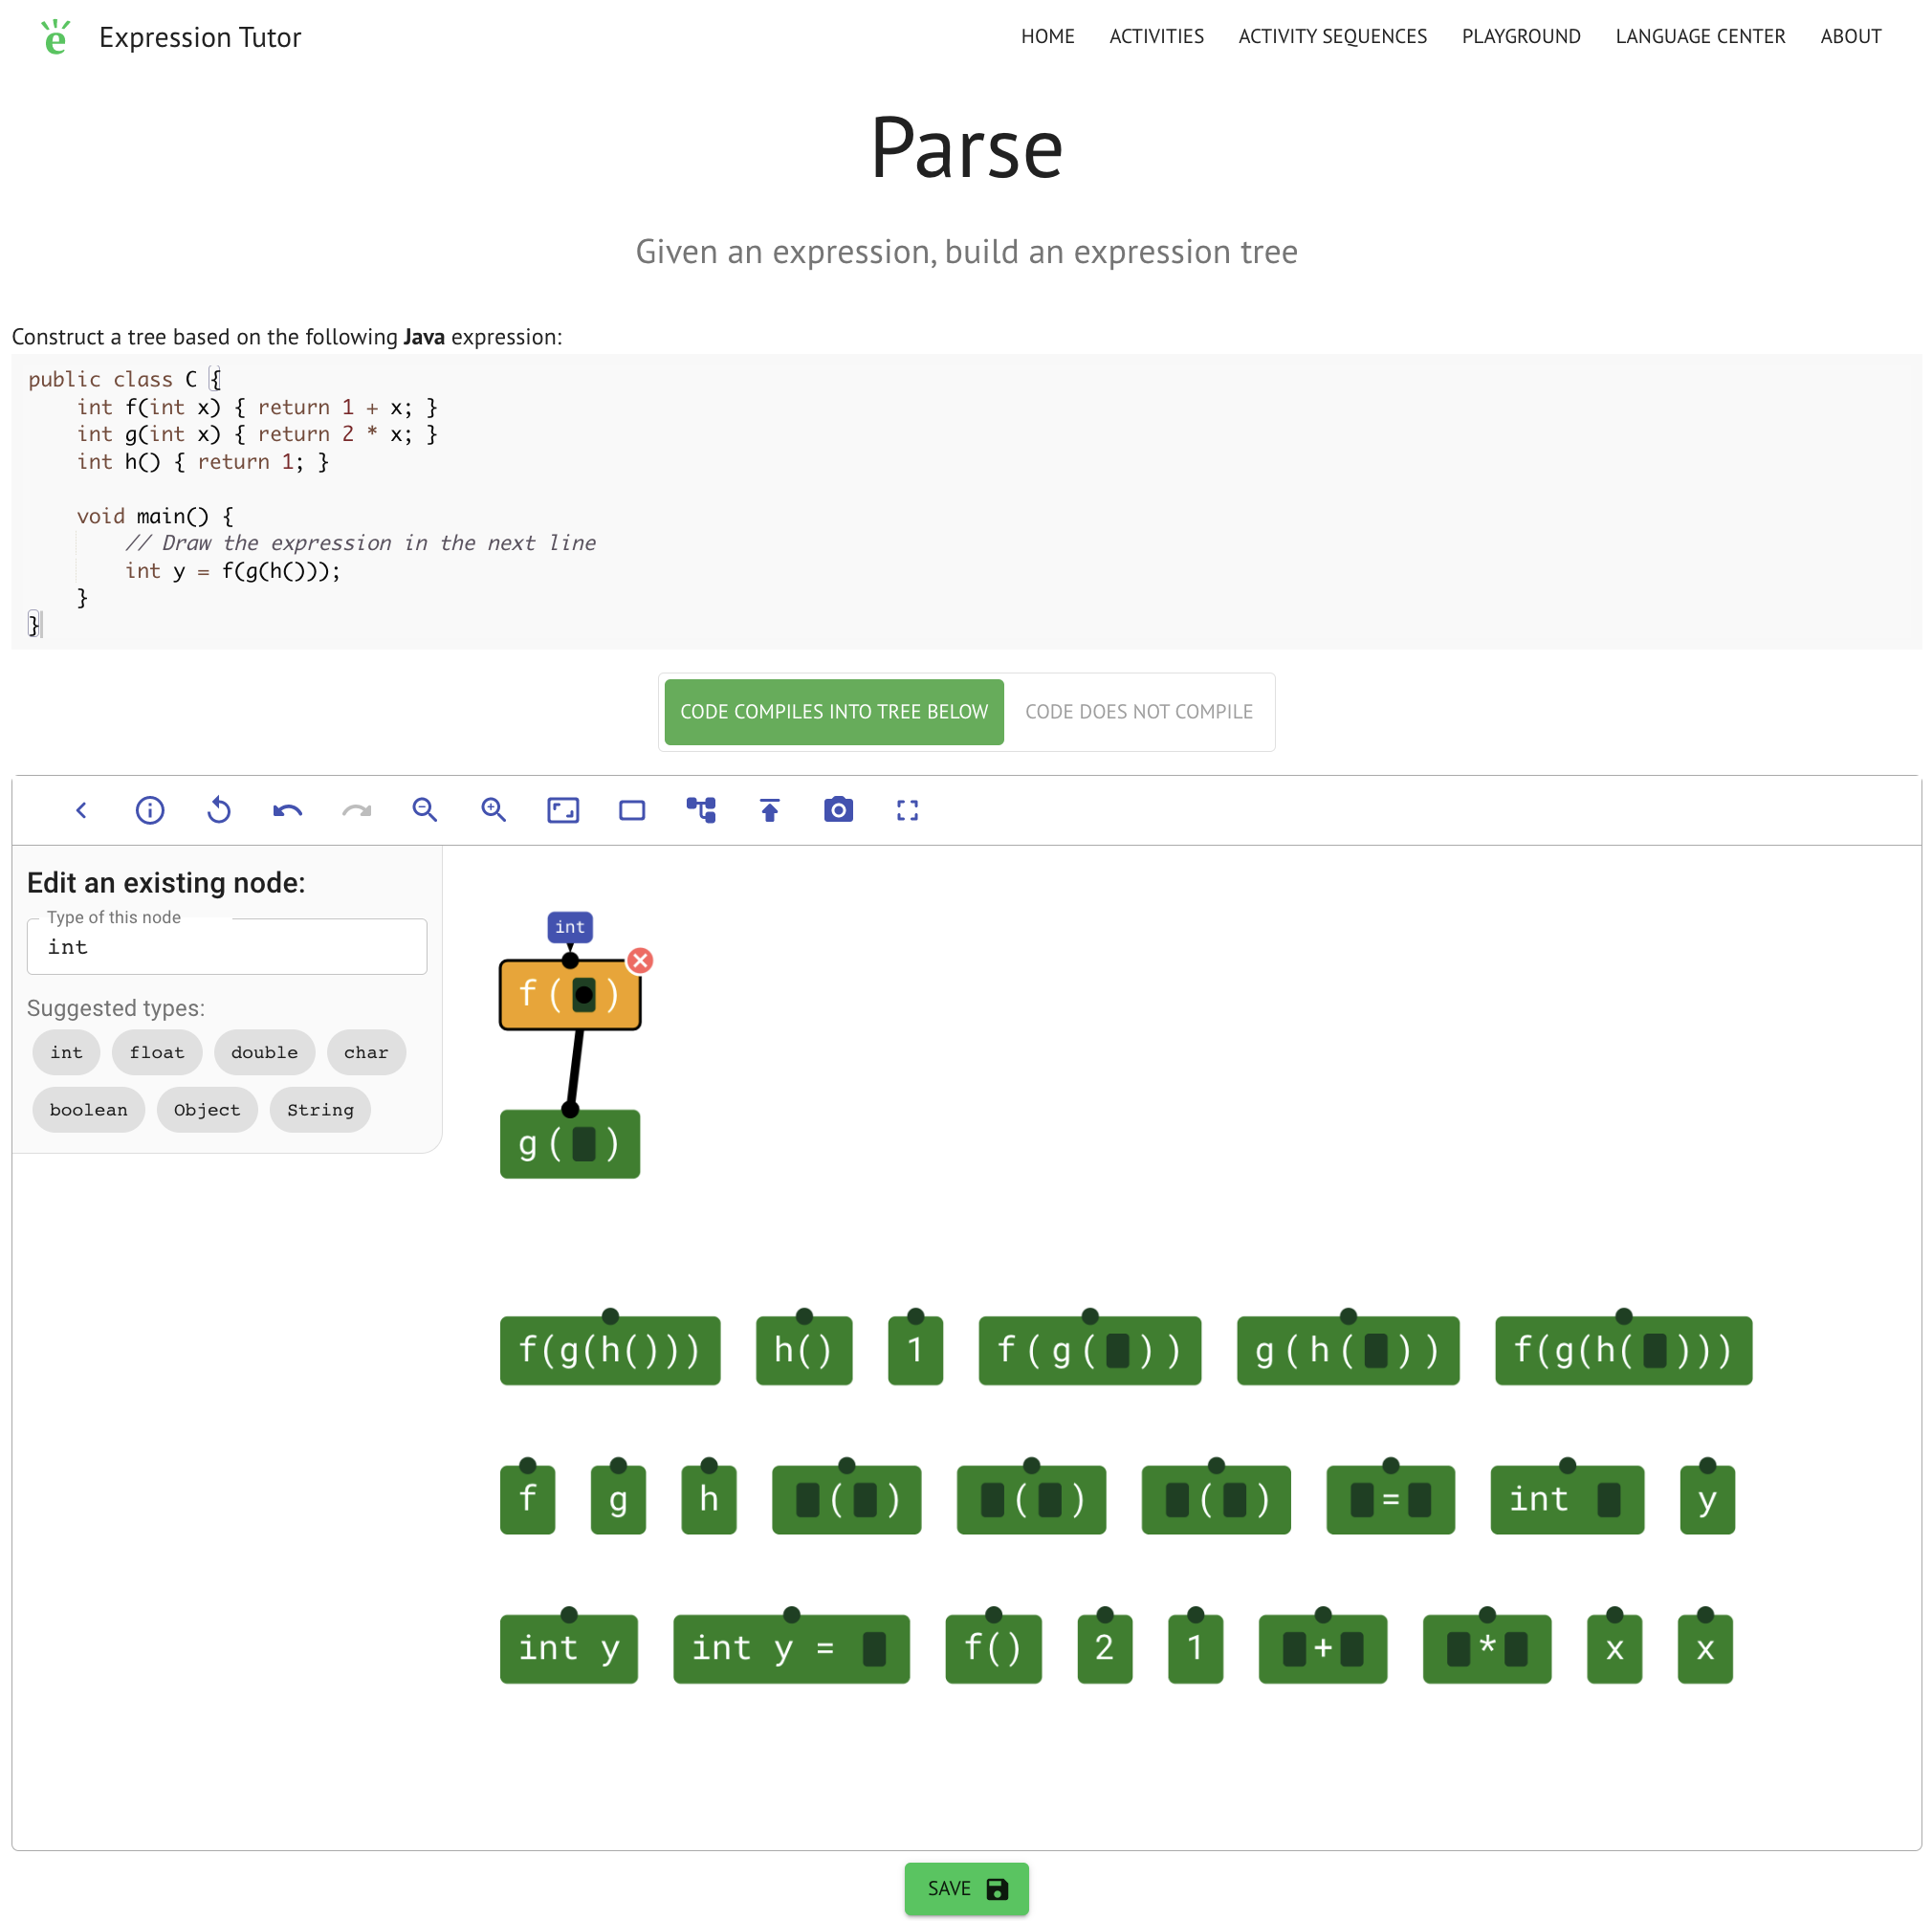
\includegraphics[width=0.6\textwidth]{res/2/et_parse_activity.png}
    \caption{Expression Tutor activity: students draw expression trees by 
selecting, connecting and annotating the correct nodes.}
    \label{fig:bg-et-activity}
\end{figure}

\subsection{Expression Service}\label{sec:bg-rw-le-et-es}

Expression Service is a collection of different stateless services used by
Expression Tutor (such as parsing and analyzing source files, producing and
ingesting expressions diagrams and generating expression from formal
grammar specifications). It can be executed either as a stand–alone command
line executable or as a web service.
All the services, with the exception of source code parsing for expression
extraction, are designed in a language–agnostic way. 
Everything operates with the common data structure (expression tree diagram) to
avoid any possible dependency on or bias towards specific
programming–languages. This also allows to simply add support for new languages
that would immediately get access to all the features the platform has to offer
as long as there exists a mapping from source code to expression tree diagram.
The latter is one of the most relevant features of Expression Service for this
document. The ability of Expression Service to analyze source code files of
selected programming languages and generate expression tree diagrams for them
serves as the cornerstone for the automatic activity generation functionality
(Chapter~\ref{sec:impl}). This mapping process from source code to expression
tree diagrams is usually accomplished by building the AST of the source code
and then all the expression constructs are \textit{visited} to build expression
trees. At the time of writing this document, the supported languages are
Java 11~\footnote{Java 17 parsing is supported but new expression constructs 
introduced after Java 11 are not fully supported yet. For this reason only
support for Java 11 is advertised.} and Python 3.11.

\subsection{Architecture}

\textbf{Figure~\ref{fig:bg-et-arch}} illustrates the high–level architecture
of the Expression Tutor platform, its main components and user interfaces.
Expression Tutor (web) exposes a number of HTTP APIs that may be used through
regular means or by using a wrapper command–line utility. It is also responsible
for storing and retrieving activities data from the database. When necessary,
it invokes Expression Service (\textbf{Section~\ref{sec:bg-rw-le-et-es}}) to
perform more advanced operations involving expressions. The components are
carefully designed to have clear responsibilities and the architecture is devoid
of any instance of circular dependency.

\begin{figure}[ht]
    \centering
    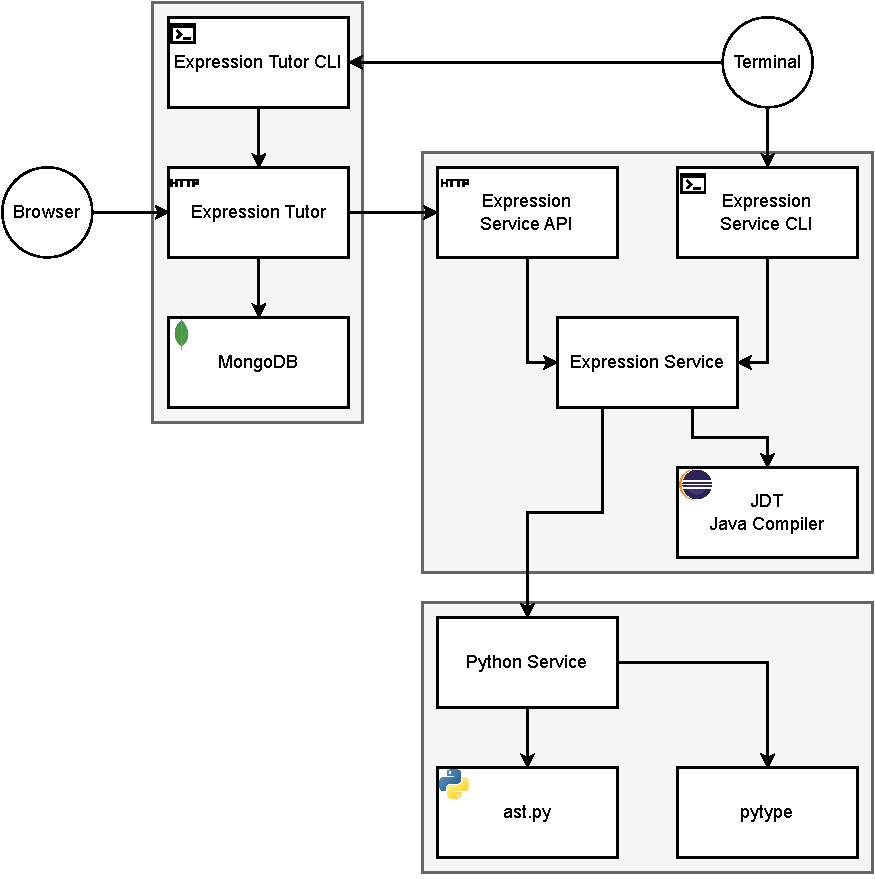
\includegraphics[width=0.6\linewidth]{res/2/et_arch.drawio.pdf}
    \caption{Architecture of the Expression Tutor platform.}
    \label{fig:bg-et-arch}
\end{figure}

\textbf{Figure~\ref{fig:bg-es-arch}} illustrates the highly modular architecture
of Expression Service. Each feature is implemented by a number of smaller 
modules to facilitate composability. This means that the different features can
be developed and updated as individual components that may be assembled
together in different ways, while minimizing the effects of the changes on
other modules.

\end{chapterBody}
